\documentclass{article}
\usepackage{amsmath}
\usepackage{tikz}
\usepackage{geometry}
\usepackage{enumerate}
\renewcommand{\labelenumi}{(\alph{enumi})}
\renewcommand{\labelenumii}{(\roman{enumii})}
\geometry{verbose,letterpaper,tmargin=2cm,bmargin=2cm,lmargin=2cm,rmargin=2cm}

\title{CS181: Bayesian Networks and HMMs}
\author{Danny Zhu \& Tianhui Cai}
\let\b\mathbf

\begin{document}
\maketitle

\section*{Problem 1}
\begin{center}
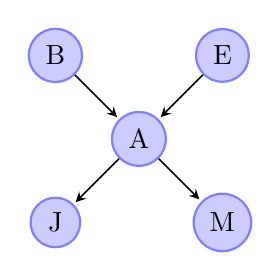
\begin{tikzpicture}[->,semithick,>=stealth,node distance=1.5cm,shorten >=1pt]
  \tikzstyle{state}=[circle,draw=blue!50,fill=blue!20,thick]
  \node [state] (B) {B};
  \node [state] (A) [below right of=B] {A};
  \node [state] (E) [above right of=A] {E};
  \node [state] (J) [below left of=A] {J};
  \node [state] (M) [below right of=A] {M};

  \path (B) edge (A)
        (E) edge (A)
        (A) edge (J)
            edge (M);
\end{tikzpicture}
\end{center}

\begin{enumerate}[(a)]
\item \textit{Let $S$ be the set of all nodes in the network. Using
  the idea of $d$-separation, for each pair of nodes $U,V\in S$, list
  the subsets of $S\setminus \{U,V\}$ that when observed would render
  $U,V$ independent.}

  \begin{tabular}{|c|c|}
  \hline
  Node pair $(U,V)$ & $S'\subset S\setminus \{U,V\},I(U,V|S')$ \\
  \hline
  $(B, A)$ & Impossible \\
  $(B, E)$ & $\emptyset$ \\
  $(B, J)$ & Any set containing $A$ \\
  $(B, M)$ & Any set containing $A$ \\
  $(E, A)$ & Impossible \\
  $(E, J)$ & Any set containing $A$ \\
  $(E, M)$ & Any set containing $A$ \\
  $(A, J)$ & Impossible \\
  $(A, M)$ & Impossible \\
  $(J, M)$ & Any set containing $A$ \\
  \hline
  \end{tabular}

\item \textit{Build another Bayesian network that has the same
  independence properties, using variable order $M,J,A,B,E$.}

  The process is to consider $M,J,A,B,E$ in order and for each node
  $N_i$ to find the minimal set of nodes $Pa(N_i)$ such that
  $P(N_i|N_1,\ldots,N_{i-1})=P(N_i|Pa(N_i))$.

  Doing this iteratively, $P(M)=P(M)$; $P(J|M)=P(J|M)$;
  $P(A|M,J)=P(A|M)$; $P(B|M,J,A)=P(B|A)$;
  $P(E|M,J,A,B)=P(E|A,B)$. Hence we get the following diagram:

  \begin{center}
    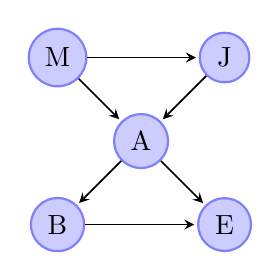
\begin{tikzpicture}[->,semithick,>=stealth,node distance=1.5cm,shorten >=1pt]
      \tikzstyle{state}=[circle,draw=blue!50,fill=blue!20,thick]
      \node [state] (B) {M};
      \node [state] (A) [below right of=B] {A};
      \node [state] (E) [above right of=A] {J};
      \node [state] (J) [below left of=A] {B};
      \node [state] (M) [below right of=A] {E};

      \path (B) edge (A)
      edge (E)
      (E) edge (A)
      (J) edge (M)
      (A) edge (J)
      edge (M);
    \end{tikzpicture}
  \end{center}
  This however doesn't actually give us all the same independence
  conditions as before: for instance, M and J are now never
  independent given any set of given nodes, whereas any set containing
  A previously would make them independent.  Hence there does not
  exist such a Bayes model with this ordering that has all the same
  independence conditions as the previous model.  This does, however,
  have the same dependence conditions as the previous model, by
  construction.
\item \textit{How many parameters are there in the BN in (a) and the
  BN in (b)?}

  (a): $1+1+4+2+2=10$.

  (b): $1+2+4+2+4=13$.

  \textit{Give three reasons why the BN in (a) is preferred over the
    BN in (b).}

  If we only care about dependence properties (which are preserved),
  \begin{enumerate}
  \item Fewer parameters means less storage.
  \item Fewer parameters means better sampling of data.
  \item No cycles $\rightarrow$ polytree $\rightarrow$ optimal
    elimination order.
  \end{enumerate}

\end{enumerate}

\section{Problem 2}
\begin{enumerate}[(a)]
\item \textit{Suppose the driver does not detect a cop and the traffic
  is slow.  Use variable elimination to determine}

  %  TODO: I'm not sure what variable elimination has to do with anything.

  \begin{enumerate}
  \item \textit{the probability of being late when the driver decides
    to speed and when the driver decides not to speed}

    $$P(OT=T|ST=T,SC=F,S)=\frac{\sum_C\sum_T P(OT=T,ST=T,SC=F,S,C,T)}{P(ST=T,SC=F,S)}$$
    First we calculate the denominator: $P(ST=T,SC=F,S)=P(ST=T,SC=F)$. ST and SC are
    independent given $C$, so the denominator equals
    \begin{align*}
    &P(ST=T,SC=F|C=T)P(C=T)+P(ST=T,SC=F|C=F)P(C=F)\\
    &=0.8\cdot 0.1+0.3\cdot 0.9=0.302
    \end{align*}
    Now we evaluate the numerator $\sum_C\sum_T P(OT=T,ST=T,SC=F,S,C,T)$.
    Rearrange terms:
    \begin{align*}
    &\sum_C P(ST=T,SC=F|C)P(C) \sum_T P(T|C,ST=T,SC=F,S)P(OT=T|T,C,ST=T,SC=F,S)\\
    &=\sum_C P(ST=T,SC=F|C)P(C) g_1(S,C)
    \end{align*}
    Where $g_1(S,C)= \sum_T P(T|C,ST=T,SC=F,S)P(OT=T|T,C,ST=T,SC=F,S)$.
    \begin{align*}
    g_1(S=T,C=T)&=0.5\cdot 0.9+0.5\cdot 0=0.45\\
    g_1(S=T,C=F)&=1\cdot 0.9+0\cdot 0=0.9\\
    g_1(S=F,C=T)&=1\cdot 0.1+0\cdot 0=0.1\\
    g_1(S=F,C=F)&=1\cdot 0.1+0\cdot 0=0.1
    \end{align*}
    Rewrite the numerator as $g_2(S)$ where
    $$g_2(S)=\sum_C P(ST=T,SC=F|C)P(C)g_1(S,C)$$
    \begin{align*}
    g_2(S=T)&=0.8\cdot 0.4\cdot 0.1\cdot 0.45+0.3\cdot 0.1\cdot 0.9\cdot 0.9=0.2574\\
    g_2(S=F)&=0.4\cdot 0.4\cdot 0.1\cdot 0.1+0.4\cdot 0.1\cdot 0.9\cdot 0.1=0.0302
    \end{align*}
    The probability of being late given speeding is $1-g_2(S=T)/0.302=0.1477$.

    The probability of being late given not speeding is $1-g_2(S=F)/0.302=0.9$.

  \item \textit{the probability of getting a ticket when the driver
    decides to speed and when the driver decides not to speed}
    \begin{align*}
    &P(T=T|ST=T,SC=F,S)\\
    &=\frac{\sum_{OT}\sum_C P(OT|T=T,C,ST=T,SC=F,S)P(T|C,ST=T,SC=F,S)P(C,ST=T,SC=F,S)}{P(ST=T,SC=F,S)}
    \end{align*}
    The denominator as before is 0.302. We rearrange the numerator as follows, noting that
    $P(OT|T=T,C,ST=T,SC=F,S)=P(OT|T=T,ST=T,SC=F)$ since $OT$ is independent of $C$ given $T$.
    \begin{align*}
    &\sum_{OT} P(OT|T=T,ST=T,SC=F,S)\sum_C P(T|C,ST=T,SC=F,S)P(ST=T,SC=F|C)P(C)\\
    &=\sum_{OT} P(OT|T=T,ST=T,SC=FS)g_1(S)
    \end{align*}
    where $g_1(S)=\sum_C P(T|C,ST=T,SC=F,S)P(ST=T,SC=F|C)P(C)$.
    \begin{align*}
    g_1(S=T)&=0.5\cdot 0.8\cdot 0.4\cdot 0.1+0\cdot 0.3\cdot 1\cdot 0.9=0.016\\
    g_2(S=F)&=0\cdot 0.8\cdot 0.4\cdot 0.1+0\cdot 0.3\cdot 1\cdot 0.9=0
    \end{align*}
    Rewrite the numerator as $g_2$, where $g_2(S)=\sum_{OT}P(OT|T=T,ST=T,SC=F,S)g_1(S)$.
    \begin{align*}
    g_2(S=T)&=0\cdot 0.016+1\cdot 0.016=0.016\\
    g_2(S=F)&=0\cdot 0+1\cdot 0=0
    \end{align*}
    Hence probability of ticket given speeding is $0.016/0.302=0.0530$.

    The probability
    of ticket given not speeding is 0.


  \item \textit{Suppose the cost of a ticket is \$150, and the cost of
    arriving late is \$10. What is the expected utility of speeding
    and not speeding?  What would be the optimal decision?}

    Speeding: $-(150\cdot 0.0530 +10\cdot 0.1477)=-9.427$

    Not speeding: $-(150\cdot 0 +10\cdot 0.9)=-9$

    It is slightly better to not speed.

  \end{enumerate}

\end{enumerate}

\section*{Problem 3}
\begin{enumerate}[(a)]
  \setcounter{enumi}2
\item
  \begin{enumerate}
  \item \emph{Define the HMM for modeling the no-momentum case in terms of
    states, observations, and the model parameters necessary.}

    There are twelve states, one for each colored square on the board.

    There are four possible observations, one for each color.

    Each state can transition to any one corresponding to an adjacent
    colored square with probability $\frac14$, or to itself with the
    remaining probability.

    Each state leads to the observation of the corresponding color
    with probability $.925$, and to each of the other colors with
    probability $.025$.
  \item \emph{Run \emph{\texttt{viterbi.py}} on the two datasets,
    \emph{\texttt{robot\_with\_momentumdata}} and
    \emph{\texttt{robot\_no\_momentum.data}}, to learn an HMM for each
    condition and also to infer the sequences of locations visited by
    the robot. Explore when, how, and why a hidden Markov model is
    successful or not in inferring the robot's true sequences. Give a
    brief writeup of what you found; include any observations about
    how well HMMs work on these problems and why. Think of
    explanations for the observations, and for failures, think of
    modifications to lead to success.}

    In general, the main assumption that we make when modeling with an
    HMM is, well, that the process satisfies the Markov assumption,
    which is that the next position of the robot is independent of
    previous positions, given the current position. We also assume
    that the transition probabilities and observation probabilities
    are the same for each time step (stationarity).

    Below is a plot of the test errors on each sequence for momentum
    and no-momentum data, sorted. Both methods produce very broadly
    (somewhat uniformly) spread out results, with two high-error
    outliers each.
    \begin{center}
      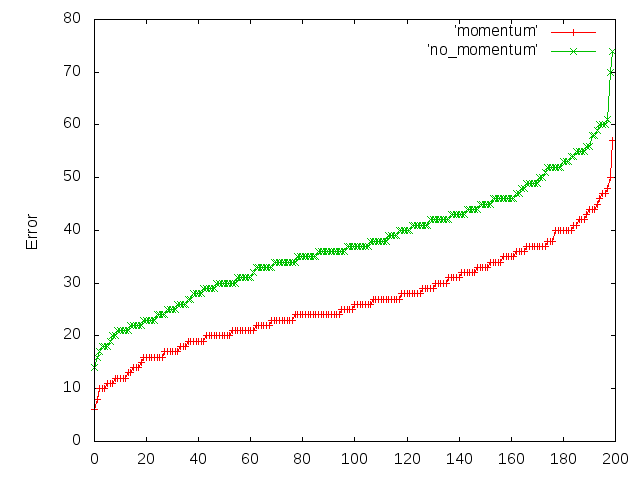
\includegraphics[scale=.5]{robot_cumul_perf.png}
    \end{center}

    For no-momentum data, the overall test performance was .8119. This
    satisfies all of our assumptions. The highest test error was 74 of
    200 states, on test sequence number 158. In this sequence, the
    robot spent two-thirds of its time in the bottom right quadrant of
    the board. Of the errors, 25 were arose from the robot being in
    3:1, but the algorithm outputting 4:2. Seven came from the reverse
    situation, altogether accounting for 32 of 74 errors. It makes
    sense that these two would be confused often, since the colors of
    the squares that are adjacent to them are similar. I think the
    particular direction of confusion is influenced by the fact that
    4:2 has only two neighbors, while 3:1 has 3. Thus, for example,
    for a sequence of moves like 3:2,3:1,4:1, the sequence 3:2,4:2,4:1
    is actually more likely.

    For momentum data, the overall test performance was .8667. In this
    case, the Markov assumption is not satisfied, since the choice of
    direction depends on the last choice of direction, whereas our
    model takes only position into account in its states. The highest
    error was 57 of 200, in test sequence number 122. Much like the
    worst case for no-momentum data, the robot spent 119 turns in the
    bottom right quadrant, and also 41 in 2:1. In this case, there
    were 11 errors of 3:1$\to$4:2 and 10 due to 3:4$\to$4:2. The first
    kind comes up for the same reason as before. The second one might
    come up because it is much less common to reach 3:4 from the
    bottom right area without momentum.

    %% \begin{itemize}
    %% \item \emph{What probabilistic assumptions are we making about the nature of
    %%   the data in using a hidden Markov model?}

    %% \item \emph{How well do these assumptions match the actual domain?}

    %% \item \emph{To what extent was, or was not, performance hurt by making such
    %%   assumptions?}

    %% \end{itemize}
  \end{enumerate}
\end{enumerate}
\section*{Problem 4}
\begin{enumerate}[(a)]
\item \emph{Describe the HMM for modeling this weather problem in terms of hidden
  states, observations, and the model parameters necessary.}

  There are hidden states corresponding to states of the world that we can't
  see. They're hidden, so (at least in this case) we don't know what they are.
  Observations are things like ``rain'', ``clouds'', ``sun'', ``fog'', etc --
  i.e., observable weather.
  The model parameters necessary are the initial probabilities of being in a
  certain state, the transition probability between states, and the probability
  of getting a particular observation given a particular states.

\item
  \begin{enumerate}
    \setcounter{enumii}2
  \item \emph{Use the two unit tests \emph{\texttt{test\_bw\_beta\_all\_equal}}
    and
    \emph{\texttt{test\_bw\_gamma\_first\_col\_equal}} to answer the following questions;
    include outputs in writeup.}

    \begin{enumerate}[(1)]
    \item \emph{Why are the betas all equal for each time step?}

      The test gives the following output:
\begin{verbatim}
beta:
[  0.333333  0.333333  0.333333  ]
[  0.333333  0.333333  0.333333  ]
[  0.333333  0.333333  0.333333  ]
[  0.333333  0.333333  0.333333  ]
[  0.333333  0.333333  0.333333  ]
[  0.333333  0.333333  0.333333  ]
[  0.333333  0.333333  0.333333  ]
[  0.333333  0.333333  0.333333  ]
[  0.333333  0.333333  0.333333  ]
[  0.333333  0.333333  0.333333  ]
\end{verbatim}

      Note that this is not a generally true fact, i.e. betas are not
      necessarily all the same in all time steps for a general HMM.  But
      in this particular case they are. The model this is run on has
      three states and a transition matrix in which every value is
      equal, i.e. the probabilities of going from any state $a$ to any
      state $b$ are all equal.  Additionally, the observation model is
      such that the probability of any given observation is equal, if we
      don't know anything about what state it's in,
      i.e. $P(O_t=o_t)=P(O_T=o_t')$.

      Now we look at the equation for $\beta$.
      \[\beta(x_t)=\sum_{x_{t+1}} P(X_{t+1}=x_{t+1}|X_t=x_t)P(O_{t+1}=o_{t+1}|X_{t+1}=x_{t+1})\beta (x_{t+1})\]
      The $\beta(x_T)$'s are initialized to all be equal, so by
      induction (we're hypothesizing that the $\beta(x_t)$'s are the
      same, always) we can pull that term out of the sum. Furthermore,
      since the transition matrix has equal entries, the first term
      $P(X_{t+1}=x_{t+1}|X_t=x_t)$ is also a constant that we can pull
      out of the sum. Then we're left with some constants times
      $\sum_{x_{t+1}} P(O_{t+1}=o_{t+1}|X_{t+1}=x_{t+1})$; by
      marginalization and the fact that $P(O_t=o_t)=P(O_t=o_t')$, this
      part is also equal across all $x_i$. Hence we have that each
      $\beta(x_i)$ at any given time period is just the product of three
      constants which are the same over all $x_i$.


    \item \emph{Why are the gamma values for the first state the same for all time periods?}

      Again, this does not appear to be a generally true fact. The outcomes
      we get from running on this simple model are as follows:

\begin{verbatim}
gamma:
[  0.333333  0.500000  0.166667  ]
[  0.333333  0.500000  0.166667  ]
[  0.333333  0.500000  0.166667  ]
[  0.333333  0.500000  0.166667  ]
[  0.333333  0.500000  0.166667  ]
[  0.333333  0.500000  0.166667  ]
[  0.333333  0.166667  0.500000  ]
[  0.333333  0.500000  0.166667  ]
[  0.333333  0.166667  0.500000  ]
[  0.333333  0.166667  0.500000  ]
[  0.333333  0.166667  0.500000  ]
[  0.333333  0.166667  0.500000  ]
\end{verbatim}

      In lecture we defined $\gamma_t(s)=P(X_t=s|O_1=o_1,\ldots,O_T=o_t)$.
      Intuitively it makes sense that $\gamma_t(s)$ are all equal, i.e. that
      the probability of the HMM being at the first state at some time $t$,
      given all observations, is the same: the transition matrix has equal
      values everywhere, so only the current $X_t$ matters rather than the
      entire sequence, and $P(O=1|X_t=1)=P(O=0|X_t=1)$, i.e. all outcomes
      are equally likely in the first state, and also they are equally likely
      if they are not in the first state. So if $\gamma_t(s)$ only depends
      on how likely we are to observe some $o_t$, and if all outcomes are
      equally likely given $x_1$ and given not-$x_1$, intuitively how likely
      the $t$th state is $x_1$ should all be the same.

      More rigorously, we can take a look at the $\alpha$ values as well,
      since $\gamma_t(s)=\frac{\alpha_t(s)\beta_t(s)}{\sum_{s'}\alpha_t(s')\beta_t(s')}$:
      since $\beta_t(s')$ is always 1/3 for all $s'$, we then just have
      \[\gamma_t(s)=\frac{\alpha_t(s)}{\sum_{s'}\alpha(t,s')}\]
      Considering the recursive formula for $\alpha$,
      \[\alpha_t(x_t)=P(o_t|x_t)\sum_{x_{t-1}}P(x_t|x_{t-1})\alpha(x_{t-1})\]
      we see that again we pull $P(x_t|x_{t-1})$ out of the sum as it is
      equal everywhere. It suffices to show
      $\alpha_t(1)/(\alpha_t(2)+\alpha_t(3))$ remains constant, i.e.
      \[\frac{P(o_t|1)\sum \alpha(x_{t-1})}{P(o_t|X_t=2)\sum\alpha(x_{t-1})+P(o_t|X_t=3)\sum \alpha(x_{t-1})}=\frac{P(o_t|X_t=1)}{P(o_t|X_t=2)+P(o_t|X_t=3)}\]
      This remains constant as $P(O_t=1|X_t=1)=P(O_t=0|X_t=1)$, and the other two
      always sum up to the same thing ($P(O_t=0|X_t=2)=P(O_t=1|X_t=3)$ and vice versa).

    \end{enumerate}

  \item \emph{Alpha and beta values get small for long sequences. If you look at the
    \emph{\texttt{get\_alpha}} function, you can see that there is normalization code.
    Why is the sum of the logs of the normalization factors the log likelihood of
    the returned observation sequence?}

    $\log(a\cdot b)=\log(a)+\log(b)$. Taking logs of small alpha and beta values
    make them less prone to encoding error.

  \end{enumerate}

\item
  \begin{enumerate}
  \item \emph{Run \texttt{\emph{classify.py}} on each data set to learn an HMM
    for each city from the training data and use them to classify the test data.
    Vary the number of hidden states from 1 to 6 and plot the final classification
    accuracy vs the number of hidden states.}

    \begin{itemize}
    \item \texttt{weather\_boston\_la.data}:\\

      \begin{tabular}{|cc|}
        \hline
        Number hidden states & Accuracy (fraction)\\
        \hline
        1 & 1.000\\
        2 & 1.000\\
        3 & 1.000\\
        4 & 1.000\\
        5 & 1.000\\
        6 & 1.000\\
        \hline
      \end{tabular}

      It appears that the difference in weather between Boston and LA are
      easily representable by an HMM, even with only one state.

    \item \texttt{weather\_boston\_sea.data}:\\

      \begin{tabular}{|cc|}
        \hline
        Number hidden states & Accuracy (fraction)\\
        \hline
        1 & 0.470\\
        2 & 0.910\\
        3 & 0.890\\
        4 & 0.900\\
        5 & 0.895\\
        6 & 0.885\\
        \hline
      \end{tabular}

      Presumably worse performance for Boston vs Seattle can be attributed
      to weather that is less obvious to classify.

    \item \texttt{weather\_all.data}:\\

      \begin{tabular}{|cc|}
        \hline
        Number hidden states & Accuracy (fraction)\\
        \hline
        1 & 0.460\\
        2 & 0.703\\
        3 & 0.667\\
        4 & 0.740\\
        5 & 0.878\\
        6 & 0.878\\
        \hline
      \end{tabular}

    \end{itemize}

  \item \emph{Plot $\log(P(D|\Theta))$ for training the model for Boston with
    varying numbers of hidden states. Do you see any patterns?}

    \begin{center}
      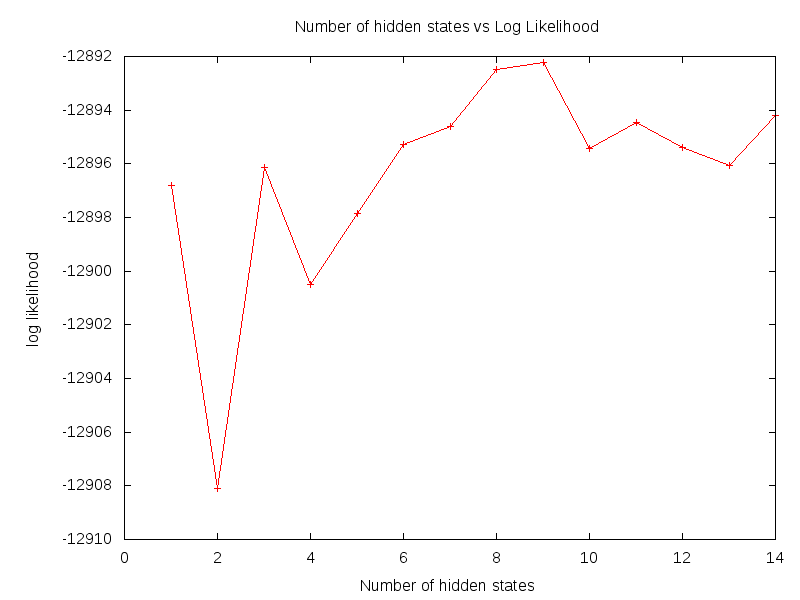
\includegraphics[scale=0.5]{4civ_plot.png}
    \end{center}

    Firstly we see that log likelihoods are all very negative, so that
    likelihood is a very small fraction. This may seem surprising
    given that even with one hidden state, the HMM classifies the test
    data perfectly. But these are so negative because log likelihood
    of a dataset is the sum of the log likelihood of each
    item. Because likelihood is (almost) never 1, i.e. log likelihood
    is always negative, we end up with the sum of a lot of negative
    numbers.  This example shows how important it is to use logs,
    since otherwise, there would be difficulty representing these
    numbers distinctly.

    As for patterns in the data, there seems to be a local maximum at
    3. It starts out around -12897 with 1 hidden state, then drops
    precipitously to -12908 with two hidden states; at 3 hidden states
    we have a local maximum with log likelihood around -12896; it
    drops again to near -12900, reaches a maximum at 9 states, and
    seems not to do much after that.

  \item \emph{By looking at the data and the learned models, try to explain your
    results. When do more hidden states help? When are they not needed? What is
    it about the observations that makes more states unnecessary?}

    As with essentially any learning process, adding more hidden
    states allows the model to capture more complexity in the
    underlying process. Eventually overfitting starts to set in.

    In general, though, we prefer simpler models even if they are
    slightly worse. Also, as a tradeoff, more hidden states means much
    more time to process, as Baum-Welch takes more time per iteration
    as well as more iterations to converge with more hidden states.

  \item \emph{The data was generated synthetically. How many hidden states do you
    think were in our generating model? Why?}

    Probably 9, since using 9 states in our HMM produced the highest likelihood.

  \end{enumerate}
\end{enumerate}
\end{document}
